\chapter{INTRODUCTION}
\label{ch:introduction}

\section{Overview}
This project presents a simulation-based autonomous indoor parcel delivery system developed using the Robot Operating System 2 (ROS 2) and the Gazebo simulation environment. The aim of the system is to model an intelligent mobile robot that can autonomously navigate indoor spaces such as university buildings, office corridors, and institutional facilities. All development, testing, and evaluation are carried out entirely in simulation, without the use of physical hardware.

The system focuses on core navigation tasks including mapping, localization, path planning, trajectory smoothing, and obstacle avoidance. An Improved A* (IA*) algorithm is used for global path planning to generate collision-free routes on occupancy grid maps. However, since grid-based planners typically produce paths with sharp turns that are difficult for differential-drive robots to follow, a spline-based path smoothing technique is applied to generate smooth and kinematically feasible trajectories. To accurately follow these trajectories, a Model Predictive Control (MPC) approach is implemented, allowing the robot to track planned paths while respecting motion and stability constraints.

The entire system is integrated within the ROS 2 framework, using standard communication mechanisms such as topics, services, and action servers to coordinate navigation and control. In addition, a web-based control interface is developed to allow users to assign delivery tasks, set goal locations, and monitor the robot’s behavior in real time during simulation. By adopting a simulation-only approach, the project enables safe and efficient testing of autonomous navigation algorithms while providing a strong foundation for future hardware implementation and real-world deployment

\section{Project idea} 
This project focuses on the development of a simulation-based autonomous indoor parcel delivery system using ROS 2. A virtual mobile robot is designed to navigate indoor environments such as university buildings and office corridors, delivering parcels without human intervention. The system emphasizes core navigation tasks including path planning, obstacle avoidance, and smooth motion control, all implemented and evaluated within a simulated environment. A simple web-based interface is provided for assigning delivery goals and monitoring system operation.

\section{Purpose of the project}
The purpose of this project is to design and evaluate a simulation-based autonomous indoor parcel delivery system using ROS 2. The project aims to develop a reliable navigation framework that allows a mobile robot to autonomously move within indoor environments while safely avoiding obstacles and following smooth, feasible paths.

By implementing and testing the system entirely in simulation, the project focuses on improving key aspects of autonomous navigation such as path planning, trajectory smoothing, and control performance. The work provides a practical software-based foundation that can support future hardware implementation and further research in autonomous indoor delivery systems.

\section{Motivation and Need of the Project}

The motivation for this project arises from the increasing demand for automation and contactless services, particularly in the post-pandemic era. Many organizations aim to minimize the physical effort involved in repetitive and labor-intensive tasks while maintaining high service quality. Shortages of labor, increasing operational costs, and the need for 24/7 service further highlight the importance of autonomous delivery systems. Moreover, in environments such as hospitals, industrial facilities, and emergency zones, human-based delivery can be risky and unsafe. Autonomous robots can operate in such conditions efficiently while supporting safer workplaces. These needs are addressed in this project by offering an effective, dependable, and user-friendly autonomous indoor parcel delivery solution designed for structured environments.
\subsection{Project Specifications}
This section presents the technical and functional specifications of the proposed User-Friendly Autonomous Parcel Delivery System with Adaptive Navigation.
The specifications define the system environment, navigation framework, control
strategy, software tools, and safety mechanisms used in the design and implementation.
\begin{table}[H]
	\centering
	\caption{System Specifications}
	\label{tab:system_specs}
	\begin{tabular}{|p{5cm}|p{9cm}|}
		\hline
		\textbf{Category} & \textbf{Specification} \\
		\hline
		System Type & Software-based autonomous indoor parcel delivery system \\
		\hline
		Operating Environment & Indoor structured environments (hospitals, offices, universities) \\
		\hline
		Robot Platform (Simulated) & Differential-drive mobile robot (TurtleBot3 Waffle model in ROS~2/Gazebo) \\
		\hline
		Navigation Framework & Custom-developed navigation stack (in-house path planning, smoothing, and control algorithms) integrated within the ROS~2 architecture \\
		\hline
		Path Planning Algorithm & Improved A* (IA*) \\
		\hline
		Path Smoothing Method & Particle Swarm Optimization (PSO) \\
		\hline
		Localization Method & SLAM-based localization (LiDAR + odometry) \\
		\hline
		Obstacle Avoidance & Real-time dynamic obstacle avoidance \\
		\hline
		Motion Control & Model Predictive Control (MPC) \\
		\hline
		Map Representation & 2D Occupancy Grid Map \\
		\hline
		Simulation Tools & Gazebo + RViz \\
		\hline
		Programming Languages & Python (ROS~2 \& Flask), Dart (Flutter UI), SQL \\
		\hline
		Development Platform & Ubuntu Linux with ROS~2 \\
		\hline
	\end{tabular}
\end{table}
The system is designed as a fully software-based autonomous delivery platform,
allowing development and testing in a simulated indoor environment before any
hardware deployment. Navigation, mapping, and task execution are handled by a
custom-developed navigation stack built entirely in-house and integrated within the
ROS~2 architecture, rather than relying on the standard Nav2 stack. An Improved A*
algorithm is used for global path planning, while Bezier curve interpolation ensures
smooth and kinematically feasible trajectories for a differential-drive robot.
SLAM-based localization with LiDAR and odometry provides accurate pose estimation,
and real-time obstacle avoidance allows safe operation in dynamic environments.
Motion control is achieved using a self-designed Model Predictive Controller (MPC),
which improves tracking accuracy and stability. A 2D occupancy grid map is used for
environment representation.
The system is implemented using Python for ROS~2 and Flask backend services,
and Dart with Flutter for the user interface. Safety features such as obstacle inflation,
collision avoidance, and emergency stop mechanisms ensure reliable and secure
operation in shared indoor spaces.

\section{Project Objectives}

\subsection{General Objectives}

The primary objective of this project is to design and implement an autonomous parcel delivery system capable of navigating indoor environments safely and efficiently. The system aims to minimize human involvement, improve delivery accuracy, and enhance operational efficiency through intelligent navigation and control.

\subsection{Specific Objectives}

The specific objectives of this project are:
\begin{itemize}
    \item To design an autonomous mobile robot capable of safe indoor navigation.
    \item To develop adaptive path planning and obstacle avoidance algorithms for dynamic environments.
    \item To implement a user-friendly application for task assignment and real-time monitoring.
    \item To evaluate system performance under different indoor scenarios.
    \item To propose a scalable architecture for future system expansion.
\end{itemize}


\section{Scope of the Project}

The scope of this project is limited to indoor parcel delivery in structured environments. The system focuses on ground-level navigation in corridors, rooms, and hallways. It includes sensing, navigation, control, and user interface design. Outdoor navigation, stair climbing, elevator integration, and heavy payload transportation are outside the scope of this project. The focus remains on achieving reliable and efficient indoor operation.

\section{Significance of the Project}

This project is significant both academically and practically. From an academic perspective, it contributes to the study of autonomous navigation, robotics, and embedded systems. It provides hands-on experience in integrating hardware and software for real-world applications.

From a practical standpoint, the proposed system offers a cost-effective and scalable solution for indoor parcel delivery. It reduces dependency on manual labor, improves efficiency, and enhances service reliability. The project also aligns with sustainable development goals by promoting innovation, smart infrastructure, and efficient resource utilization.

\section{Applications of the Proposed System}

\subsection{Hospitals}

The autonomous parcel delivery system can be used to transport medicines, lab samples, medical records, and equipment between departments. This reduces the workload on healthcare staff and minimizes human contact in sensitive areas. Timely delivery improves patient care and operational efficiency. The robot can safely navigate corridors with staff and patients present.
\subsection{University Campuses}
On large campuses, the system can deliver documents, books, and equipment between offices, libraries, and laboratories. It reduces delays caused by long walking distances and limited staff availability. The robot supports efficient inter-departmental operations and helps automate internal logistics. Real-time tracking ensures transparency and accountability.

\subsection{Office Buildings}
Within a corporate setting, the robot is able to take care of the internal mail, files, and small packages.
vertical- between departments and floors. This enhances better workflow and minimizes disruption to a minimum.
employees. The system provides safe and quality delivery of crucial documents.

\begin{figure}[H]
\centering
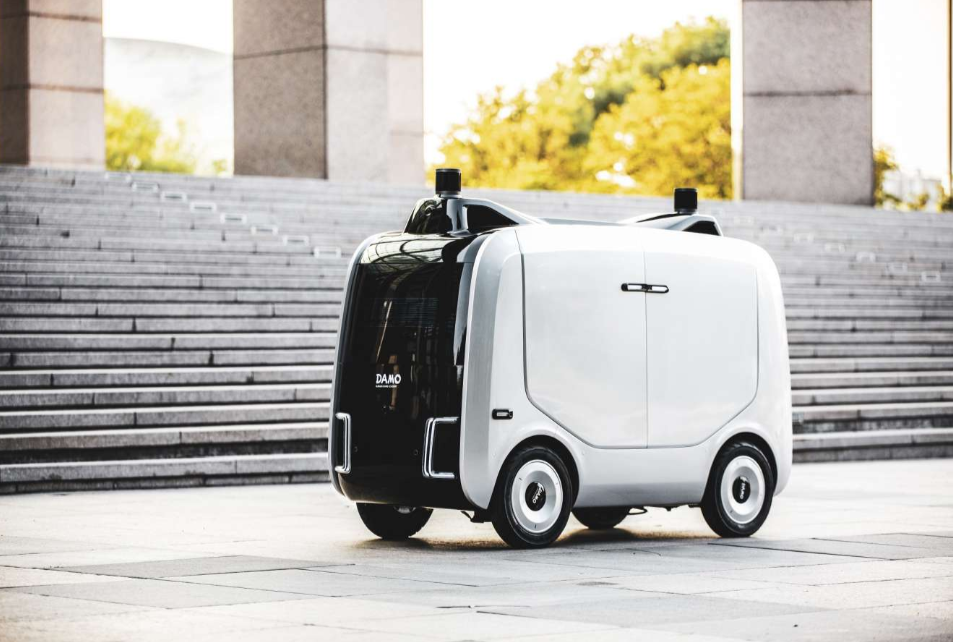
\includegraphics[width=0.55\textwidth]{delivery.png}
\caption{Example of an autonomous parcel delivery \cite{simonite2017hungry}}
\label{fig:delivery}
\end{figure}


\subsection{Industrial Units}
The robot is capable of moving tools, components and materials between work stations in factory floors. This minimises the amount of manual operation and accelerates the production. The system promotes the principles of automation and lean manufacturing. It also enhances safety because there is minimization of unnecessary human movement in hazardous areas.

\subsection{Hotels}
In hotels, the system can deliver room service items, laundry, and guest amenities. This enhances guest experience by providing fast and contactless service. The robot operates quietly in hallways and common areas. It also helps reduce staff workload during peak hours.

\subsection{Emergency and Disaster Zones}
In hazardous indoor environments, the robot can deliver essential supplies where human access is risky. It supports rescue operations by carrying tools, food, or medical kits. The system improves safety by reducing human exposure to dangerous conditions. Autonomous navigation ensures reliable operation in unstable environments.


\section{Limitations of the System}

Although the proposed system offers numerous advantages, it has certain limitations. The robot’s performance depends on sensor accuracy, battery capacity, and environmental conditions. The system is designed for flat indoor surfaces and may not perform effectively on stairs or uneven terrain. Network connectivity issues may affect real-time monitoring. These limitations provide direction for future improvements.

\section{Project Plan}
The following table shows the proposed project plan and timeline. The entire project, spanning literature review, algorithm development, web interface implementation, and full ROS 2/Gazebo simulation integration, was successfully completed within a total duration of \textbf{32 weeks}.

\begin{table}[H]
	\centering
	\caption{Proposed Project Plan and Timeline}
	\label{tab:project_plan}
	\begin{tabular}{|c|p{6cm}|c|p{5cm}|}
		\hline
		\textbf{S\#} & \textbf{Tasks} & \textbf{Duration} & \textbf{Resource Person} \\
		\hline
		1 & Literature Review & 02 Weeks & M.Ali, Aitzaz Arshad, Gulfam Haider \\
		\hline
		2 & Path Planning (A*/IA*) + Pruning & 02 Weeks & M.Ali, Aitzaz Arshad, Gulfam Haider \\
		\hline
		3 & Path Smoothing (PSO + Cubic Spline) & 02 Weeks & M.Ali, Aitzaz Arshad \\
		\hline
		4 & Model Predictive Control (MPC) Design \& Implementation & 02 Weeks & Aitzaz Arshad, Gulfam Haider \\
		\hline
		5 & Cellular Decomposition \& Dynamic Programming Integration & 02 Weeks & M.Ali, Aitzaz Arshad, Gulfam Haider \\
		\hline
		6 & Web Interface -- Frontend Development (Flutter) & 03 Weeks & M.Ali, Aitzaz Arshad \\
		\hline
		7 & Web Interface -- Backend Development (Flask) \& API Integration & 04 Weeks & M.Ali, Aitzaz Arshad \\
		\hline
		8 & ROS 2 Jazzy Installation \& Virtual Environment Configuration & 01 Week & M.Ali, Aitzaz Arshad, Gulfam Haider \\
		\hline
		9 & Gazebo Simulation World Design (Multi-Room Delivery Environment) & 02 Weeks & M.Ali, Aitzaz Arshad, Gulfam Haider \\
		\hline
		10 & SLAM Implementation \& Occupancy Grid Mapping & 01 Week & M.Ali, Aitzaz Arshad, Gulfam Haider \\
		\hline
		11 & Porting Path Planning, Smoothing \& MPC Algorithms into ROS 2/Gazebo Simulation & 03 Weeks & M.Ali, Aitzaz Arshad, Gulfam Haider \\
		\hline
		12 & Web -- Gazebo -- ROS 2 Full System Integration & 03 Weeks & M.Ali, Aitzaz Arshad \\
		\hline
		13 & System Testing \& Performance Evaluation & 02 Weeks & Aitzaz Arshad, Gulfam Haider \\
		\hline
		14 & Documentation \& Final Report Writing & 03 Weeks & M.Ali, Aitzaz Arshad, Gulfam Haider \\
		\hline
	\end{tabular}
\end{table}

\section{Project Timeline}
The following figure shows the Gantt chart for the project schedule, covering the complete 32-week duration of the project.
\begin{figure}[H]
	\centering
	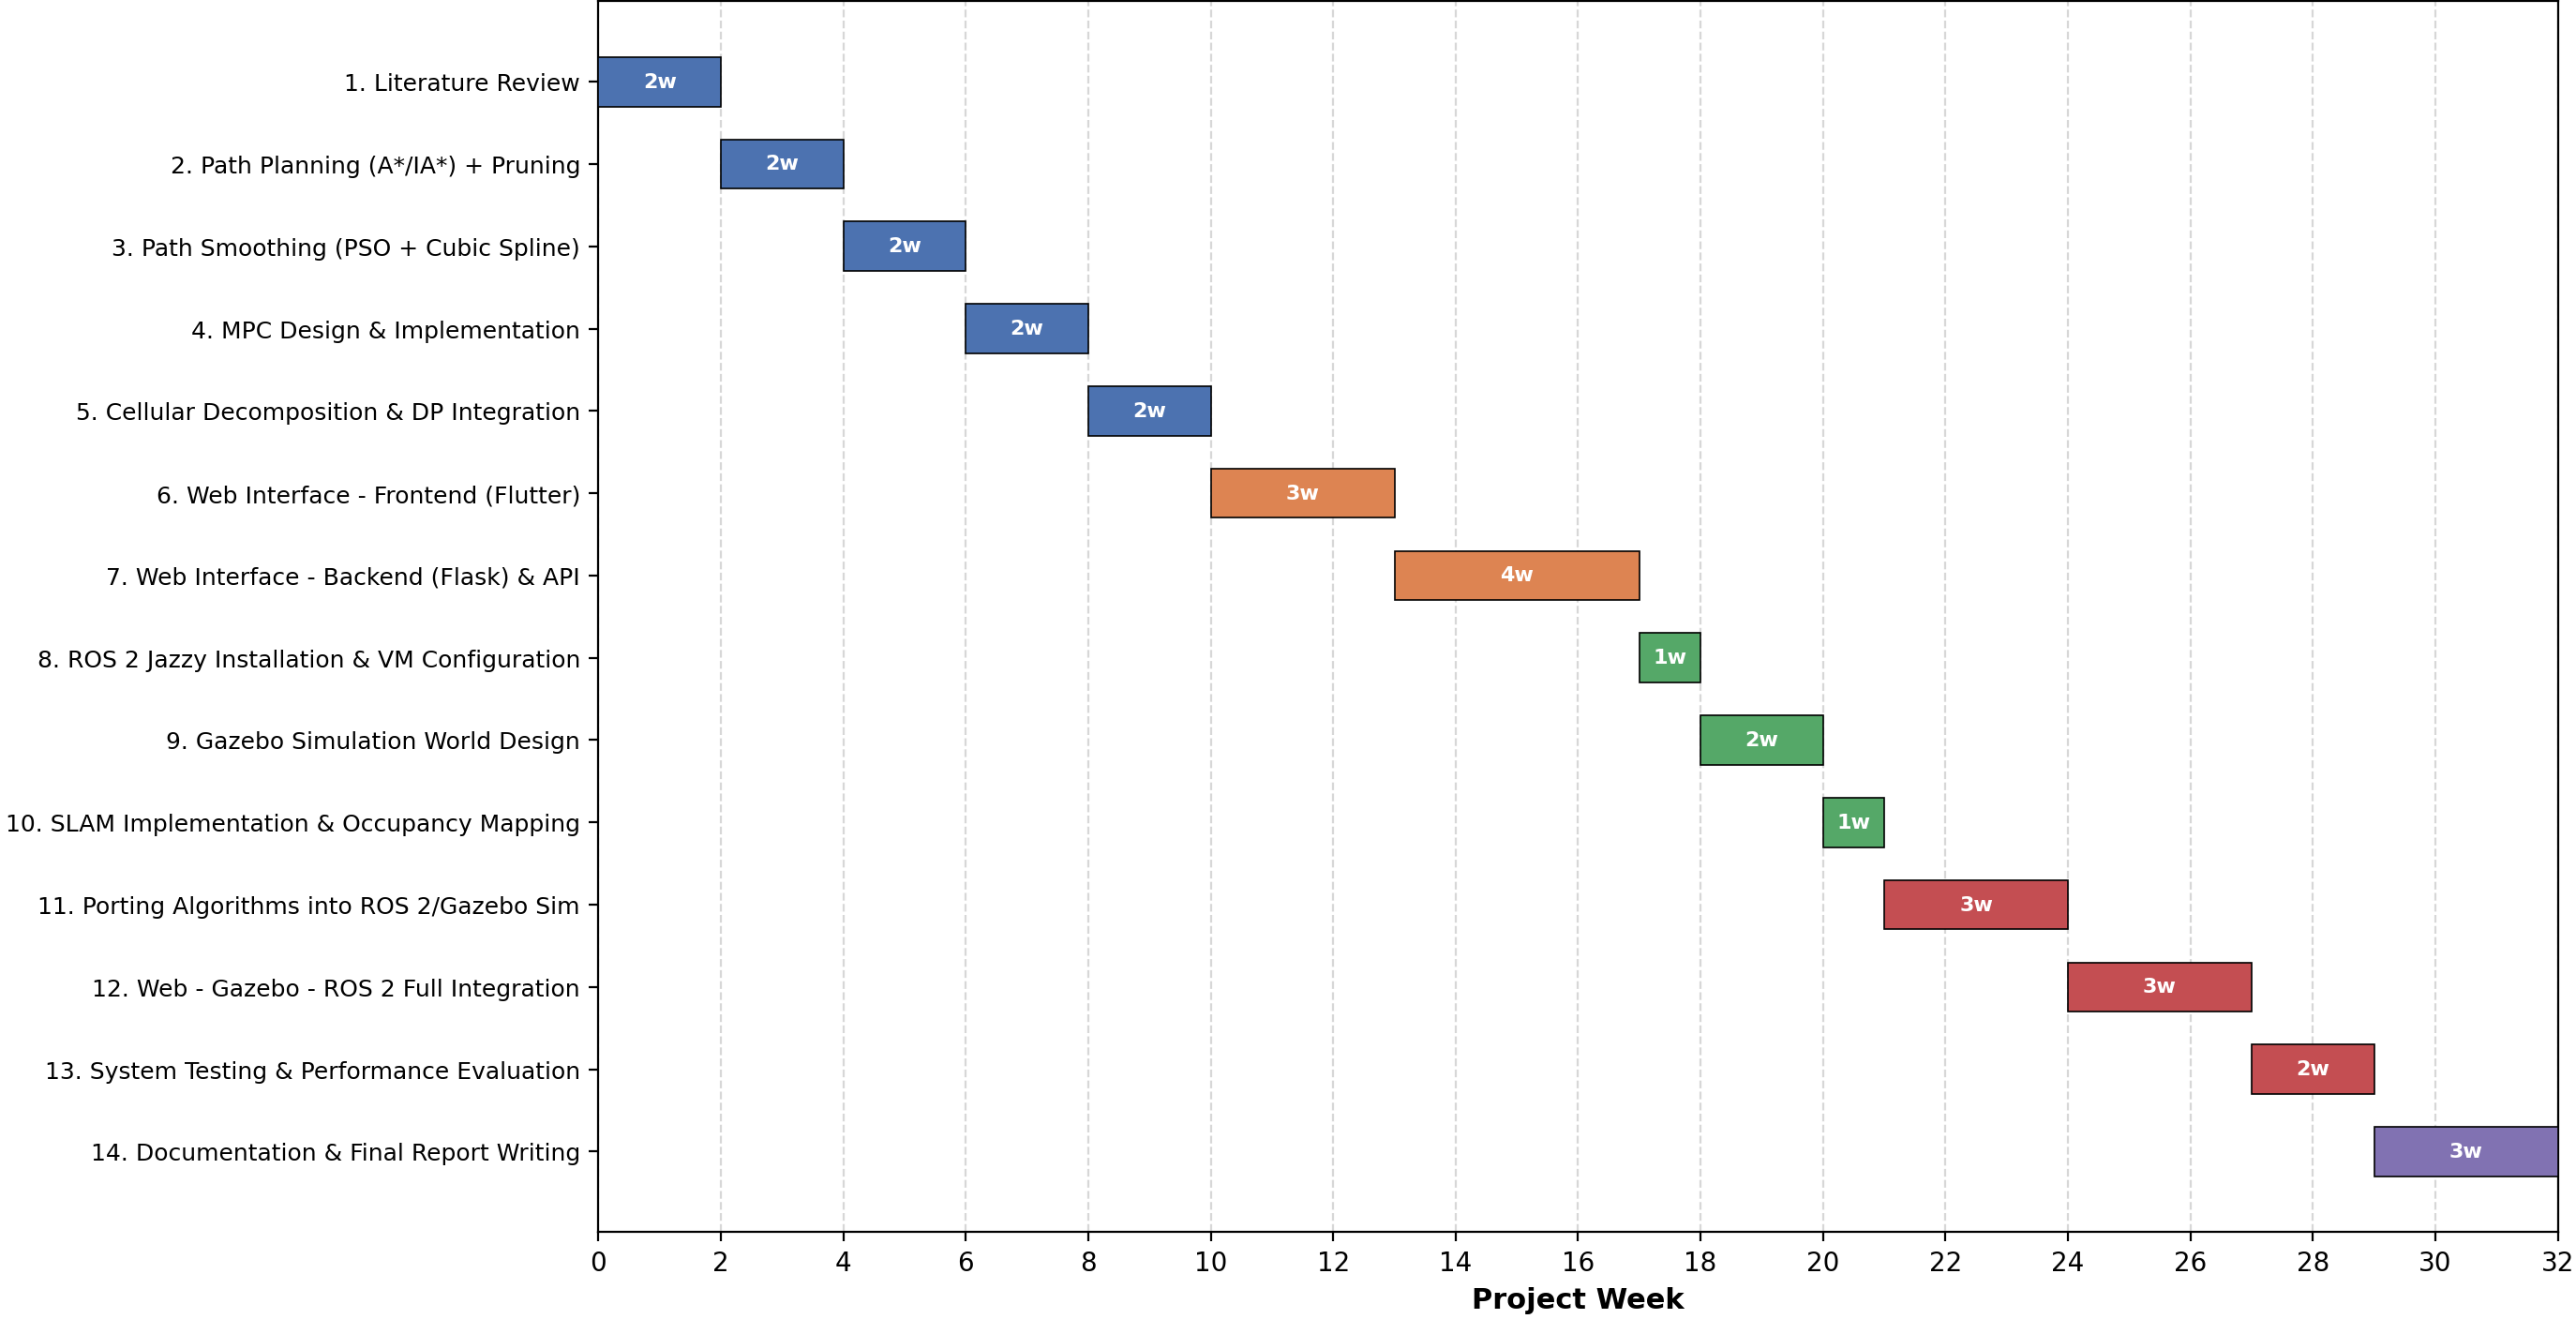
\includegraphics[width=1.0\textwidth]{chart.png}
	\caption{Project Timeline (Gantt Chart)}
	\label{fig:gantt_chart}
\end{figure}

\subsection{Targeted Sustainable Development Goals}

This project aligns with the United Nations Sustainable Development Goals (SDGs) by addressing key challenges in healthcare logistics, education, infrastructure innovation, and sustainable community living. The specific SDGs targeted by the Autonomous Parcel Delivery System are detailed in Table \ref{tab:sdgs}.

\begin{table}[h]
\centering
\caption{List of Targeted Sustainable Development Goals}
\label{tab:sdgs}
\renewcommand{\arraystretch}{1.5} % Adds vertical padding for better readability
\begin{tabular}{|c|p{0.25\textwidth}|c|p{0.45\textwidth}|}
\hline
\textbf{S\#} & \textbf{Targeted SDGs} & \textbf{SDG No.} & \textbf{Implementation Detail} \\ \hline
1 & Good Health and Well-Being & SDG \#3 & 
Autonomously transports medical supplies and lab reports in hospitals, reducing staff workload and minimizing human contact to lower cross-contamination risks. \\ \hline
2 & Quality Education & SDG \#4 & 
Supports academic operations on university campuses by efficiently delivering documents, assignments, and equipment between faculty offices, libraries, and laboratories. \\ \hline
3 & Industry, Innovation, and Infrastructure & SDG \#9 & 
Develops a scalable autonomous delivery architecture using ROS~2 to modernize internal logistics in warehouses and commercial buildings. \\ \hline
4 & Sustainable Cities and Communities & SDG \#11 & 
Promotes smart community living in universities and offices by reducing congestion and improving operational efficiency through automated delivery. \\ \hline
\end{tabular}
\end{table}\section{Report Organization}
The report is structured to provide a clear understanding of the project from background to results. Chapter 1 introduces the project, including its motivation, objectives, specifications, and scope. Chapter 2 reviews existing literature on path planning algorithms, mobile robot control strategies, ROS 2 navigation architecture, and previous implementations, highlighting gaps in current approaches. Chapter 3 explains the design and implementation of the custom navigation system, covering the IA* path planning algorithm, path smoothing methods, motion controller design, and ROS 2 integration. Chapter 4 describes the tools and techniques used, including the TurtleBot3 hardware, ROS 2 framework, Gazebo simulation, Python programming, and RViz visualization. Chapter 5 presents project results and evaluation, discussing navigation performance, tracking accuracy, path quality, web interface and Ros.Chapter 6 provides the conclusion and future work, summarizing achievements, lessons learned, limitations, and recommendations for enhancements like dynamic obstacle handling, multi-robot coordination, and real-world deployment. Chapter 7 relates the project to Sustainable Development Goals (SDGs), showing how autonomous navigation contributes to innovation, sustainable cities, and responsible production. Finally, Chapter 7 provides the conclusion and future work, summarizing achievements, lessons learned, limitations, and recommendations for enhancements like dynamic obstacle handling, multi-robot coordination, and real-world deployment.

\section{Chapter Summary}

This chapter provided a comprehensive introduction to the user-friendly autonomous parcel delivery system. It discussed the background, motivation, problem statement, proposed solution, objectives, scope, significance, applications, limitations, and project milestones. The chapter establishes a strong foundation for the technical and analytical discussions presented in the subsequent chapters.